%!TEX TS-program = xelatex
\documentclass[10pt,twoside,BCOR12mm,DIV11,headinclude=false,footinclude=false,titlepage=true]{scrartcl}

%%

%\usepackage{makeidx}
%\makeindex

%%%%%%%%%%%%%%%%%%%%%%%%%%%%%%%%%%%%%%%
%
%    FONTS   % % % 
%
%%%%%%%%%%%%%%%%%%%%%%%%%%%%%%%%%%%%%%%

\usepackage{fontspec}


%%%

\setromanfont[Mapping=tex-text]{Cambria}
\setsansfont{Helvetica Neue Light}
\setmonofont[Scale=MatchLowercase]{Menlo}
\newfontfamily\devfont[Renderer=Graphite,Script=Devanagari,Language=Sanskrit]{Annapurna SIL}
\newfontfamily\devhfont[Script=Devanagari,Language=Sanskrit]{Kohinoor Devanagari Regular}
\newfontfamily\bangfont[Script=Bengali,Language=Bengali]{Bangla MN}
\newfontfamily\orifont[Script=Oriya,Language=Oriya]{Oriya MN}
\newfontfamily\telfont[Script=Telugu,Language=Telugu]{Telugu MN}


\newfontinstance\devbfont[Renderer=Graphite,Script=Devanagari,Language=Sanskrit]{Annapurna SIL Bold}
\newfontinstance\devhmfont[Script=Devanagari,Language=Sanskrit]{Kohinoor Devanagari Medium}
\newfontinstance\devhbfont[Script=Devanagari,Language=Sanskrit]{Kohinoor Devanagari Bold}

\newcommand{\scb}[1]{\textbf{\textsc{#1}}}
\newcommand{\infont}[1]{\textsc{\scriptsize #1}}
\newcommand{\embf}[1]{\textbf{\emph{#1}}}
\newcommand{\echov}[1]{\textrm{\scriptsize #1}}
%%%%%%%%%%%%%%%%%%%%%%%%%%%%%%%%%%%%%%%%
%
%    PAGE LAYOUT   % % %
%
%%%%%%%%%%%%%%%%%%%%%%%%%%%%%%%%%%%%%%%%

\typearea[current]{classic}
\usepackage[headsepline,automark]{scrpage2}

% * GENERAL PAGE LAYOUT SETTINGS * * * * * * * * * * * * * * * * * * * * * * 

\setkomafont{pagenumber}{\normalfont\sffamily\bfseries}

\newcommand{\myversion}{\begin{scriptsize}Lazarus Project (Cologne Sanskrit Lexicon) Project Documentation 1\end{scriptsize}}



% * * FXRU HEADINGS * * * * * * * * * * * * * * * * * * * * * * * * * * * * * * *

\newpagestyle{fxruheadings}{%
{\rightmark\hfill}%
{\hfill\rightmark}%
{\hfill}%
(\textwidth, .4pt)}%
{%
{\pagemark \quad \vline \quad \hfill  \myversion}%
{\myversion\hfill \quad \vline \quad \pagemark}%
{\hfill\pagemark \hfill}%
}

% * * FXRU LEX HEADINGS * * * * * * * * * * * * * * * * * * * * * * * * * * * * * * *

% TO DO


% * * FXRU APPENDIX HEADINGS * * * * * * * * * * * * * * * * * * * * * * * * * * * * * * *

\newpagestyle{fxrutextheadings}{%
{\rightmark\hfill}%
{\hfill\rightmark}%
{\hfill}%
(\textwidth, .4pt)}%
{%
{\pagemark \quad \vline \quad  \textit{\rightmark} \hfill  \myversion}%
{ \myversion\hfill \textit{\rightmark} \quad \vline \quad \pagemark}%
{\hfill\pagemark \hfill}%
}


%%

%\usepackage[headsepline,automark]{scrpage2}
%\pagestyle{scrheadings}
\pagestyle{fxruheadings}
\automark[chapter]{subsection}
\pagenumbering{arabic}



% LAYOUT STRUCTURE %%%%%%%%%%%%%%%%%%%%%%%%%%%%

\setcounter{secnumdepth}{5}
\setcounter{tocdepth}{5}

%%%%%%%%%%%%%%%%%%%%%%%%%%%%%%%%%%%%%%%%%
%%%%%%%%%%%%%%%%%%%%%%%%%%%%%%%%%%%%%%%%%

%  OTHER PACKAGES       %%%%%%%%%%%%%%%%%%%%%%%%%%%%

\usepackage{rotating}
\usepackage{multicol}
\usepackage{natbib}
\usepackage{graphicx}


%Test features%%%%%%%%%%%%%%%%%%%%%%%%%%%%%%
\usepackage{xltxtra}
\usepackage{hyperref}
\hypersetup{								%
unicode=true,								%
pdftex, 										%
colorlinks=true, 							% 
linkcolor=black,  						%
citecolor=black, 							%
filecolor=black,  							%
pagecolor=, 								%
urlcolor=black,  							%
pdftitle={Vedic Accent and Lexicography}, 	%
pdfauthor={Felix Rau} 				%
}

\def\partautorefname{part}
\def\chapterautorefname{\S}
\def\sectionautorefname{\S}
\def\subsectionautorefname{\S}
\def\subsubsectionautorefname{\S}
\def\paragraphautorefname{\S}

%%%%%%
\usepackage{gb4e}



\begin{document}

\subject{
\includegraphics[width=4cm]{cdsl-logo.png}}
\title{{\devhbfont ऌ} l̥ and {\devhbfont लृ} lr̥ in Sanskrit Lexicography}
\author{Felix Rau}
\date{}
\publishers{University of Cologne – Lazarus Project}
\uppertitleback{{\bfseries {\devhmfont ऌ} l̥ and {\devhmfont लृ} lr̥ in Sanskrit Lexicography}\\ {\bfseries Lazarus Project: Cologne Sanskrit Lexicon, Project Documentation 1}\\ \\ \includegraphics[width=2cm]{by.eps} This work is licensed under the Creative Commons Attribution 4.0 International License.\\ \\ cite as: Rau, Felix 2017. \emph{{\devhmfont ऌ} l̥ and {\devhmfont लृ} lr̥ in Sanskrit Lexicography.} Lazarus Project: Cologne Sanskrit Lexicon, Project Documentation 1. Cologne: Lazarus Project. \href{https://doi.org/10.5281/zenodo.837257}{doi:10.5281/zenodo.837257}}
\lowertitleback{Lazarus Project (Cologne Sanskrit Lexicon)\\ University of Cologne\\ http://www.cceh.uni-koeln.de/lazarus\\ http://www.sanskrit-lexicon.uni-koeln.de/\\}
\maketitle

\section{Introduction}
This report documents the graphematic representation of the vocalic L (Devanagari: {\devfont ऌ}/ ISO 15919: l̥) and the combination of consonantal L with vocalic R (Devanagari: {\devfont लृ}/ ISO 15919: lr̥) in Sanskrit lexicography. 

\section{{\devhmfont ऌ} l̥ and {\devhmfont लृ} lr̥}

Vocalic L is represented by a simple vowel letter {\devfont ऌ} in Devanagari, while the combination of consonantal L with vocalic R is represented by the akṣara {\devfont लृ}. Although these two are clearly distinct entities, they were conflated in the original digitisation of the Cologne Sanskrit Lexicon (CSL).\footnote{http://www.sanskrit-lexicon.uni-koeln.de/} However, a closer look shows that problems of inconsistent treatment of {\devfont ऌ} l̥ and {\devfont लृ} lr̥ have a long and distinguished tradition in the writing systems used in modern Sanskrit lexicography. The relevant writing systems in this context are Devanagari and Latin script. Of the various Latin-based transliteration systems, four are considered in this report: The ISO standard ISO 15919:2001, the transliteration used in \citet{mw72,mw}, the Sanskrit Library Phonetic Basic encoding scheme (SLP1), and the popular Harvard-Kyoto transliteration system.

\subsection{The vowel {\devhmfont ऌ} l̥}

Vocalic L {\devfont ऌ} l̥  belongs to a group of linguistically controversial graphemes (and ultimately phonemes) of Sanskrit. This controversial group of graphemes in Sanskrit scripts consists of the long vocalic R {\devfont ॠ} r̥̄, the vocalic L {\devfont ऌ} l̥, and in particularly the long vocalic L {\devfont ॡ} l̥̄. Indologists have treated these graphemes with suspicion. Böhtlingk and Roth avoided  {\devfont ऋ} r̥, {\devfont ॠ} r̥̄, and {\devfont ऌ} l̥ in verbal forms by replacing them with their guṇa forms \emph{ar}, \emph{ār}, and \emph{al} in the entries of the Großes Petersburger Wörterbuch \citep{pwg}. \citet{mw72} groups these three graphemes in one section “{\devfont ॠ} {\devfont ऌ} {\devfont ॡ}” and prefixes this section with the following paragraph:

\begin{quote}
No Sanskrit word begins with any of these vowels; ṛī [{\devfont ॠ} r̥̄] appears only in the Gen[itive] plur[al] of nouns terminating in ṛi [{\devfont ऋ} r̥], in the acc[usative] plur[al] of fem[inine] nouns of relationship, and in the nom[inative] and acc[usative] plur[al] of neuter nouns in ṛi. As to the vowel lṛi [{\devfont {\devfont ऌ}} l̥] it occurs only in some forms of the root klṛip [{\devfont कॢप्} kl̥p]. The long lṛī [{\devfont ॡ} l̥̄] is a mere invention of grammarians.	
\end{quote}


This text is missing from \citet{mw} where each of the three letters has its own section. As \citet{mw72} states, vocalic L {\devfont ऌ} l̥ is rare in Sanskrit words and nearly exclusively occurs in forms of the root {\devfont कॢप्} kl̥p ‘to be well ordered’. Other occurrences are doubtful or artificial. The only possible occurrence is in the root {\devfont कॢब्} kl̥b ‘accomplishment’ which is suspiciously close to  {\devfont कॢप्} kl̥p. Several dictionaries list the proper name {\devfont ऌतक} l̥taka. However, this form is generally considered to be a mispronunciation of {\devfont ऋतक} r̥taka by these lexicographers. The lemma {\devfont ऌ} l̥ ‘the earth, the mother of the gods’ is secondary lemma from tantric texts derived from the vowel  {\devfont ऌ} l̥. Other entries containing {\devfont ऌ} l̥ concern the letter and sound {\devfont ऌ} l̥ itself and derivations of it: {\devfont ऌकार} l̥kāra and {\devfont ऌवर्ण} l̥varṇa both meaning ‘the sound {\devfont ऌ} l̥’.

\subsection{The akṣara {\devhmfont लृ} lr̥}

The akṣara {\devfont लृ} lr̥ – the combination of the consonant {\devfont ल} l with the vowel {\devfont ऋ} r̥ — is even less common. The only well-attested entries that contain {\devfont लृ} lr̥ are not for lexemes in the strict sense, but for technical terms derived from inflectional affixes. \citet{mw72} gives the following definitions:

\begin{quote}
{\devbfont लृङ्} lr̥ṅ ‘a technical term or symbol for the terminations of the Conditional or for that Mood itself.’ 

{\devbfont लृट्} lr̥ṭ ‘a technical term or symbol for the terminations of the Second Future or for that Tense itself.’ 
\end{quote}


The various dictionaries differ slightly in their treatment of these technical terms from Pāṇini. The dictionnaire sanscrit-français \citep{stc} has both {\devfont लृङ्} lr̥ṅ and {\devfont लृट्} lr̥ṭ  in romanisation and Apte’s Sanskrit English Dictionary \citep{ap90} lists {\devfont लृङ्} lr̥ṅ and {\devfont लृट्} lr̥ṭ in Devanagari. \citet{ccs,cae}  and \citet{md} only have an entry for {\devfont लृट} lr̥ṭ. In contrast to \citet{mw72}, \citet{mw} has an entry for {\devfont लृट्} lr̥ṭ, but instead of {\devfont लृङ्} lr̥ṅ, the \citet{mw} edition gives {\devfont लृ} lr̥ ‘N[ame]. of the terminations of the Conditional Mood or N[ame] of that Mood itself’ as an entry, although he lists {\devfont लृङ्} lr̥ṅ and {\devfont लृट्} lr̥ṭ – not {\devfont लृ} lr̥ – under the entry {\devfont ल} la. 

Apte in his Sanskrit English Dictionary (1890) is particularly inconsistent in his treatment of {\devfont ऌ} l̥ and {\devfont लृ} lr̥. Under the entry {\devfont ऌ} l̥, he states that “No Sanskrit word begins with l̥ or l̥̄, except some of the technical names of Pâṇini for tenses and moods; e. g.~ḷṅ [l̥ṅ] and ḷṭ [l̥ṭ].” However, {\devfont लृङ्} lṛṅ  and {\devfont लृट्} lṛṭ are clearly instances of {\devfont लृ} lṛ with a consonantal onset and \citet{ap90} himself lists them correctly under the consonant {\devfont ल} l in the same dictionary.

The only proper lexeme reported to contain the combination {\devfont लृ} lr̥ is absent from all major lexicographic works such as the Große Petersburger Wörterbuch \citep{pwg} and \citet{mw72,mw}.  However, \citet{wil}, \citet{yat}, and the \citet{shs} contain an entry for a root {\devfont लृञ्च} lr̥ñc with the meaning ‘to put away’. All three dictionaries give the additional form {\devfont लृञ्चति}  lr̥ñcati. Neither of these dictionaries give references to occurrences and it is unclear where and in which particular form or forms this lexeme is attested. In particular, whether the lexeme is attested in its base form {\devfont लृञ्च} lr̥ñc or a guṇa form (presumably {\devfont लर्ञ्च} larñc) would be relevant. The three entries read as follows:

\begin{quote}
{\devbfont लृञ्च} r.~1st cl.~({\devfont लृञ्चति} ) To put away. \citep[][p.~722]{wil}

{\devbfont लृञ्च} {\devfont लृञ्चति}  1.~a.~To put away. \citep[][p.~646]{yat}

{\devbfont लृञ्च} r.~1st cl.~({\devfont लृञ्चति} ) To put away. \citep[][p.~619]{shs}
\end{quote}

\citet{shs} is based on \citet{wil}. So the fact that it occurs in both works with an identical entry is no surprise. Whether Yates has also taken this lemma from Wilson or whether he did verify it independently is unknown. The lack of entries for this lexeme in later works and especially in \citet{pwg} and \citet{mw} is suspicious and suggests that it only occurs in late varieties of Sanskrit, if it is genuine at all.

\section{Conflating {\devhmfont ऌ} l̥ and {\devhmfont लृ} lr̥}
\subsection{Conflating {\devhmfont ऌ} l̥ and {\devhmfont लृ} lr̥ in Devanagari} 

The confusion or conflation of {\devfont ऌ} l̥  and {\devfont लृ} lr̥ occurs throughout Sanskrit lexicography and probably beyond that throughout the whole philological tradition. The two glyphs {\devfont लृ} and {\devfont ऌ} are very similar in shape in Devanagari script, with {\devfont ऌ} l̥ looking very much like a frozen combination of {\devfont ल} l and {\devfont ◌ृ}, the diacritical form of {\devfont ऋ} r̥. Some cuts of Devanagari typefaces seem to make no distinction in shape between  {\devfont लृ} lr̥ and {\devfont ऌ} l̥ or at least the distinction was blurred in the usage of these typefaces. Apte’s discussion of {\devfont लृट्} lṛṭ and {\devfont लृङ्} lṛṅ under {\devfont ऌ} l̥  (see above) is a clear instance of this confusion.

The similarity is shape between {\devfont ऌ} l̥ and {\devfont लृ} lr̥ is particularly striking in Devanagari. Other Brahmi-derived scripts display far less or virtually no likeness between the two graphemes as the Table \ref{tab:indic} shows. 

\begin{table}[!h]
\begin{center}
\begin{tabular}{lll}
&l̥&lr̥\\
Devanagari&{\devfont ऌ}&{\devfont लृ}\\
Bengali&{\bangfont ঌ}&{\bangfont লৃ}\\
Oriya&{\orifont ଌ}&{\orifont ଲୃ}\\
Telugu&{\telfont ఌ}&{\telfont లృ}\\
\end{tabular}
\end{center}
\caption[l̥ and lr̥ in different Indic scripts]{\label{tab:indic}l̥ and lr̥ in different Indic scripts}
\end{table}


\subsection{Conflating {\devhmfont ऌ} l̥ and {\devhmfont लृ} lr̥ in Latin script}

The ISO standard 15919:2001 clearly distinguishes between the two and  transliterates {\devfont ऌ} as l̥ and {\devfont लृ} as lr̥ (\texttt{l} for {\devfont ल} and \texttt{r̥} for {\devfont ऋ}). The romanisation used in \citet{mw72,mw} conflates the two. The combination {\devfont लृ} lr̥ is transliterated as \texttt{lṛi} – as a combination of \texttt{l} for {\devfont ल} l and \texttt{ṛi} for {\devfont ऋ} r̥. The vowel {\devfont ऌ} l̥ is represented by the complex sequence \texttt{lṛi}, unfortunately  identical to the juxtaposition of \texttt{l} and \texttt{ṛi}. The \emph{Sanskrit Library Phonetic Basic encoding scheme} (SLP1) as defined in \citet{ScharfHyman2011} treats Sanskrit Sounds – and by that Devanagari characters – very consistently. The combination {\devfont लृ} lr̥ is encoded as \texttt{lf} – as a combination of \texttt{l} for {\devfont ल} l and \texttt{f} for {\devfont ऋ} r̥ – while the simple vowel {\devfont ऌ} l̥ is encoded by the simplex \texttt{x}. The very popular romanisation system Harvard-Kyoto conflates {\devfont लृ} lr̥ and {\devfont ऌ} l̥. In the Harvard-Kyoto system, {\devfont लृ} lr̥  is transliterated as  \texttt{lR} – as a combination of \texttt{l} for {\devfont ल} l and \texttt{R} for {\devfont ऋ} r̥. The vowel {\devfont ऌ} l̥  is represented by the combined \texttt{lR}, unfortunately again identical to the juxtaposition of \texttt{l} and \texttt{R}. All four transliteration systems are given in Table \ref{tab:latin}. 

\begin{table}[!h]
\begin{center}
\begin{tabular}{lll}
&{\devfont ऌ}&{\devfont लृ}\\
ISO & l̥ & lr̥\\
MW & lṛi & lṛi\\
SLP1 & x & lf\\
HK & lR & lR\\
\end{tabular}
\end{center}
\caption[l̥ and lr̥ in different transliterations]{\label{tab:latin}l̥ and lr̥ in different transliterations}
\end{table}

\section{Conclusion}

The vocalic L {\devfont ऌ} l̥ and akṣara or grapheme combination {\devfont लृ} lr̥ are marginal to the Sanskrit language and entries containing the two graphemes are of questionable status. However, both  {\devfont लृ} lr̥ and {\devfont ऌ} l̥ are part of Sanskrit or at least of the traditional and modern analysis and representation of the Sanskrit language. Lexicographic works that aim at representing the complete lexical knowledge concerning the Sanskrit language have to distinguish the two consistently to be faithful to this tradition.

For Sanskrit lexicography this means that systems used to represent Sanskrit have to encode the difference between the {\devfont ऌ} l̥ and {\devfont लृ} lr̥ unambiguously. While Indic writing systems such as Devanagari fulfill this requirement, some Latin-based systems fail in this regard. In particular the transliteration employed in the most widely used Sanskrit-English dictionary \citep{mw} conflates {\devfont ऌ} l̥ and {\devfont लृ} lr̥, as does the most popular Latin-based transliteration, Harvard-Kyoto. SLP 1 \citep{ScharfHyman2011} and ISO 15919 accomplish an unequivocal transliteration of Sanskrit and are much better suited for lexicographical work.




\bibliographystyle{linquiry2}
\bibliography{CSL.bib}

\end{document}
